\subsubsection{21.11.14 (Соревнования)}

\begin{center}
	1-ый день соревнований "Робофест-Юг"
\end{center}
Сегодняшний день был посвящен тренировочным матчам
\newline
Внесенные доработки:
\begin{enumerate}
	\item Было обнаружено, что  маленькие мячи попадают под колеса робота, в следствие чего теряется управление. Для предотвращения таких ситуаций была установлена защита колес.
	\begin{figure}[H]
		\begin{minipage}[h]{0.9\linewidth}
			\center{\includegraphics[scale=0.4]{days/21.11.14/images/01}}
		\end{minipage}
		\caption{Защита колес от шаров}
	\end{figure}			
	\item Из-за неисправности сервопривода был переделан МЗК.
	\begin{figure}[H]
		\begin{minipage}[h]{0.9\linewidth}
			\center{\includegraphics[scale=0.5]{days/21.11.14/images/02}}
		\end{minipage}
		\caption{Переделаный МЗК}
	\end{figure}		
	\item Была установлена Samanta и проведена одна тренировка на соревновательном поле.
	\begin{figure}[H]
		\begin{minipage}[h]{1\linewidth}
			\center{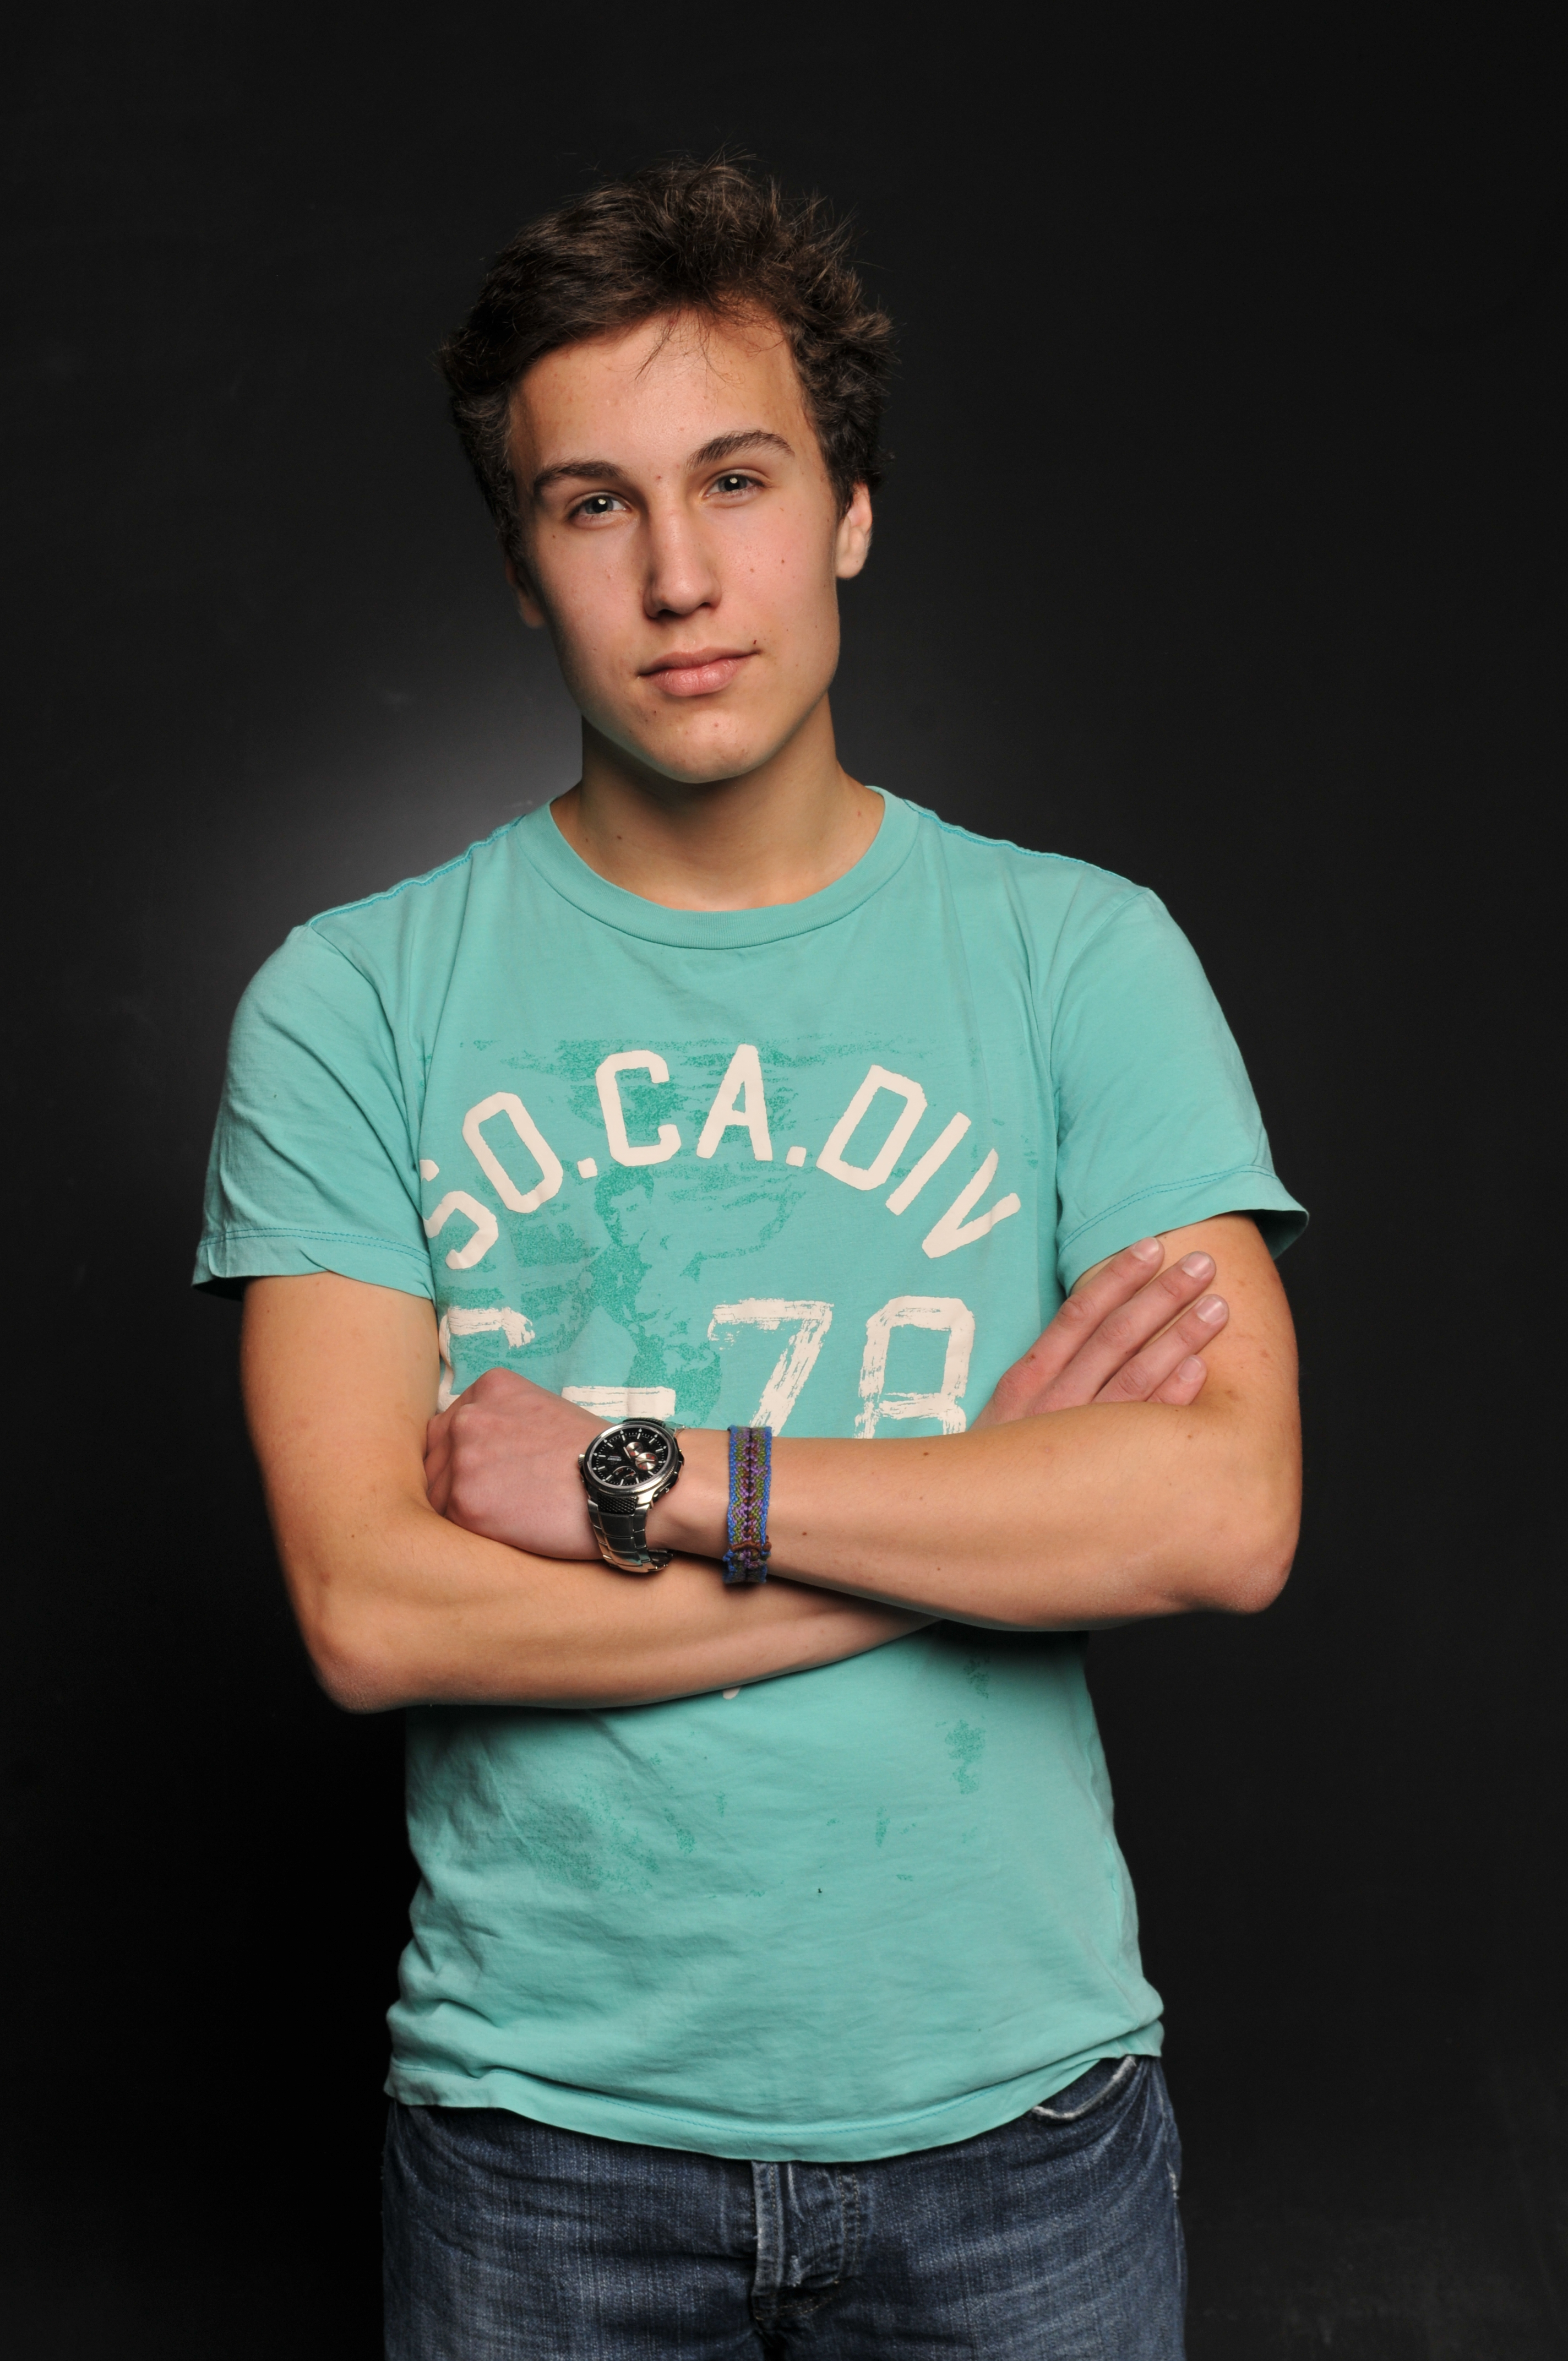
\includegraphics[scale=0.5]{days/21.11.14/images/03}}
		\end{minipage}
		\caption{Крепление Samanta}
	\end{figure}	
\end{enumerate}

\fillpage